\chapter{Denial-of-Service attacks} \label{chap:dos_attacks}

\iffalse
IN DOS, SHOW THE STATE DIAGRAMS FOR THE THINGS I MODIFIED

Cfr protocol implementation chapter for references. It is in rr/mm/cm.


for imsi detach, check att flag. detach is required for both network,
yet it doesn't work on one of them. Try with tmsi?


!!!!!!!!!!!!!!!!TALK ABOUT HOW IT INFLUENCES GPRS AS WELL!!!!!!!!!!!!!!!!!!

    Insist on the implementation and explanation, this
    is the product. Afak, no other publication explaining all the
    available attacks. insist of implementation with mobile, this is new
    and innovative to exploit normal stuff. try to explain teh method
    and give it a nice name. how i tried to solve the pb and implement
    eth code.

\fi

    \proj{OsmocomBB} makes it easy for anyone to send arbitrary messages
    to the network, and this offers various possibilities for \gls{dos}
    attacks. They are four main attacks allowing a \gls{dos} on the GSM
    network and an implementation is proposed for the first three.

    The implementations proposed here are based on the \prog{mobile}
    application of \proj{OsmocomBB} which aims to implement all the
    functions of a normal mobile phone and is introduced
    in~\Cref{chap:protocol_stack_implementation}. It is probably not the
    best choice for attacks relying on sending a high rate of messages
    to the network if the goal is purely efficiency, but these
    implementations are interesting here because they demonstrate that a
    \gls{dos} attack can be performed with some simple modifications of
    normal phone procedures and functions. \fref{fig:mobile_dos} shows
    the \gls{dos} commands added to the \prog{mobile} interface. All
    these commands provide a description and an interactive help in the
    program, and \Sref{app:tuto} of the appendices describe their
    installation and usage.

      \begin{figure}[h]
        \centering
        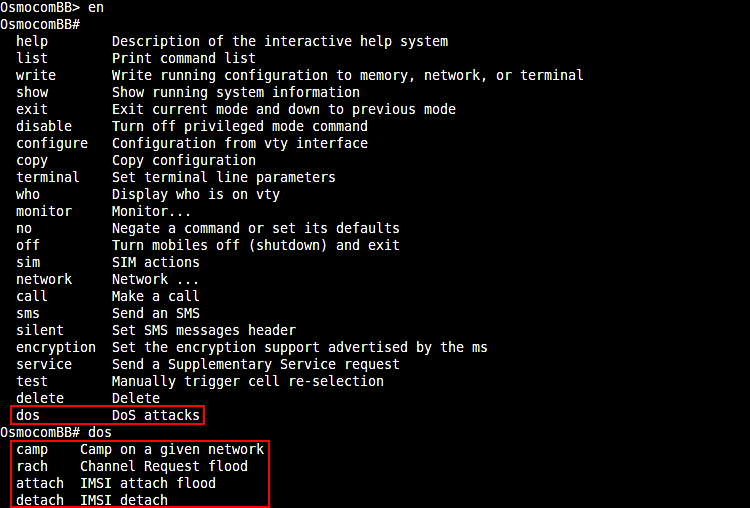
\includegraphics[width=\textwidth]{mobile_dos}
        \caption{\gls{dos} commands available in the interface of the patched \prog{mobile}
        application.}
        \label{fig:mobile_dos}
      \end{figure}

    The first section is dedicated to the RACHell attack, the second one
    to the \gls{imsi} attach attack, the third one to the \gls{imsi}
    detach attack, and the last one to attacks exploiting paging race
    conditions. Each section proposes a theoretical explanation of the
    related attack followed by an explanation of a proposed
    implementation, and a demonstration of the command usage.

    \section{RACHell}

      \subsection{Theory}

      Even if the theory had been known before, this attack was first
      demonstrated by \name{Dieter Spaar} at DeepSec in 2009 using a
      TSM30 mobile phone, the ancestor of
      \proj{OsmocomBB}~\cite{spaar_practical_2009}. It takes place very
      early in the communication process between the \gls{ms} and the
      network, since it exploits the Channel Request messages that the
      \gls{ms} sends on the \gls{rach}. This means that the phone did
      not send any identification information to the network yet, and
      that the authentication did not take place, which makes this
      attack hard to prevent.

      The channel request process, called the immediate assignment
      procedure, is summarized here but explained in more details
      in~\Sref{sec:rr_proc}. The \gls{ms} sends a Channel Request
      message on the \gls{rach} to the network. Upon reception, the
      network establishes a channel and sends an Immediate Assignment
      message to the \gls{ms}. This message contains the necessary
      information about the newly activated dedicated channel. Two
      things are interesting here. Firstly, the authentication is only
      done on this dedicated channel, after the channel establishment.
      Secondly, the network starts a timer when it receives a channel
      request, and if nothing happens on the channel, it is released
      when that timer elapses.

      The attack is simple since it floods the network with Channel
      Request messages. This has several consequences. Firstly,
      collisions on the channel are possible since the \gls{rach} uses a
      slotted ALOHA approach. Thus, it might prevent legitimate requests
      to even access the network in that cell by effectively jamming the
      channel. Secondly, each cell only has a given number of channels
      to allocate. If it receives more channel requests than that during
      the time needed for the release timer to elapse, this attack will
      exhaust them all. This makes it very difficult for a legitimate
      user to request a channel on that cell, but does not influence
      already existing connections.
      
      \subsection{Implementation}
      \label{sec:rachell_impl}

      The implementation of the RACHell attack proposed for this thesis
      is based on the \prog{mobile} application of \proj{OsmocomBB}. The
      normal behavior of this application is explained
      in~\Sref{sec:rr_proc}. When trying to establish a channel, this
      application will send a given amount of Channel Request messages.
      It stops either when an Immediate Assignment message matching this
      request is received, or when the maximum amount of requests
      allowed by the network is reached.       

      Therefore, two modifications are applied to the \prog{mobile}
      application. The first one consists of significantly increasing
      the maximum amount of requests that are sent before aborting the
      establishment attempt. The second one makes sure that the function
      matching the Immediate Assignment reference never succeeds. These
      modifications force the \gls{ms} to send a continuous flow of
      Channel Request messages to the network. A patch adding the
      \prog{dos rach} command to the \prog{mobile} application is
      available in \Sref{app:patches} of the appendices.

      This attack will target the network on which the \gls{ms} is
      currently camping. Usually, when an \gls{ms} running the
      \prog{mobile} application decides to camp on a network, it will
      start a location update procedure. If this procedure fails, the
      \gls{ms} will camp on the most suitable cell, which might not be
      part of the targeted network. Therefore, the \prog{dos camp}
      command was developed to make the phone believe that the location
      update procedure was already done, and is thus not necessary
      anymore. This makes the phone camp on the targeted network. A
      patch adding this command is available in \Sref{app:patches} of
      the appendices as well.

      To apply a \gls{dos}, it might be good to allow the cell
      reselection process to happen. For example, if the attacker
      follows the victim, the attacker's \gls{ms} will probably
      automatically select the same cell as the victim's \gls{ms} and
      thus deny service to the appropriate one. When the goal is to deny
      service to a given \gls{arfcn}, it is possible to use the
      \prog{stick} command available in the normal \prog{mobile}
      application.

      Others have implemented this attacks, for example \name{the grugq}
      at Black Hat 2010~\cite{the_grugq_base_2010}. Even if the request
      flood is supposed to impact a cell only, he reported taking down a
      \gls{bsc}. An implementation using OsmocomBB as well as some
      measurements were also proposed by Maxim
      Suraev~\cite{suraev_denial--service_2011}.

      \iffalse
need to show example of use and output
maybe in appendices
\fi

      \subsection{Demonstration}
<<<<<<< HEAD
=======
      \label{sec:rachell_demo}
>>>>>>> public
      
      Several figures displaying the various steps of the attacks and
      their output are available. The use of the \prog{dos camp}
      command, as well as the available arguments, is shown on
      \fref{fig:mobile_dos_camp}. \fref{fig:log_dos_camp0} shows how the
      \gls{ms} firsts camps on any cell when no \gls{sim} is inserted.
      \fref{fig:log_dos_camp} shows how the \prog{dos camp} command
      exploits the software \gls{sim} feature to force the \gls{ms} to
      select the requested \gls{plmn}, \comp{Telenor} in this case. A
      location update procedure would be rejected by the network, since
      the \gls{sim} is not valid. Therefore, the \prog{dos camp} command
      tricks the \gls{ms} into considering that the location update is
      not required, as shown on \fref{fig:log_dos_camp2}.

      \begin{figure}[p]
        \centering
        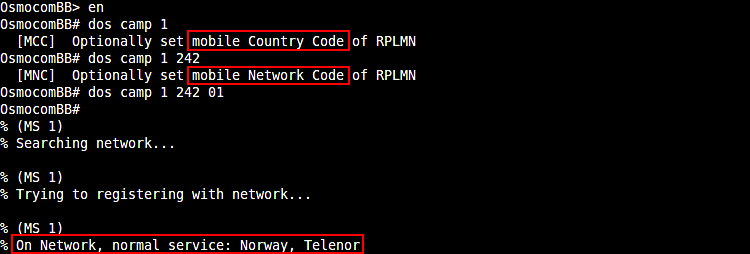
\includegraphics[width=\textwidth]{mobile_dos_camp}
        \caption{Using the \prog{dos camp} command to trick the mobile
        into camping on \comp{Telenor}}
        \label{fig:mobile_dos_camp}
      \end{figure}

      \begin{figure}[p]
        \centering
        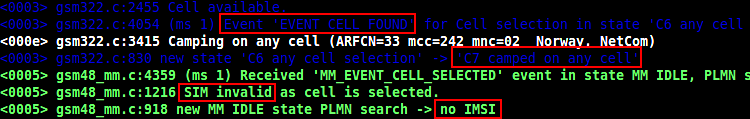
\includegraphics[width=\textwidth]{log_dos_camp0}
        \caption{Using the \prog{dos camp} command: when no SIM is
        inserted, the MS will camp on any cell.}
        \label{fig:log_dos_camp0}
      \end{figure}
     
      \begin{figure}[p]
        \centering
        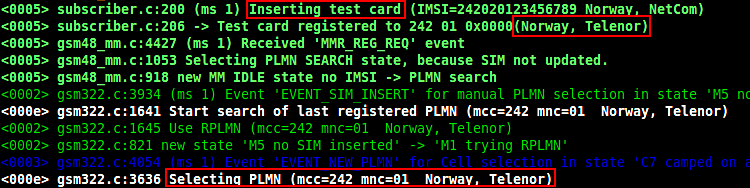
\includegraphics[width=\textwidth]{log_dos_camp}
        \caption{Using the \prog{dos camp} command: using the soft SIM
        functionality to force the MS to select the requested PLMN.}
        \label{fig:log_dos_camp}
      \end{figure}

      \begin{figure}[p]
        \centering
        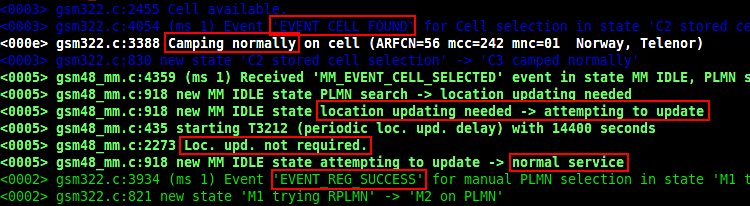
\includegraphics[width=\textwidth]{log_dos_camp2}
        \caption{Using the \prog{dos camp} command: tricking the MS into
        considering that the location update is not required.}
        \label{fig:log_dos_camp2}
      \end{figure}

      \fref{fig:mobile_dos_rach} shows the use of the \prog{dos camp}
      command in the interface of the \prog{mobile} application to camp
      on the \comp{Netcom} network, and the use of the \prog{dos rach}
      command to send three Channel Request messages to this network.
      Three messages does not constitute a \gls{dos}, but the point is
      not to damage the networks. The logs of the mobile application
      show the effect of the command. \fref{fig:log_dos_rach} shows how
      the \gls{rr} sublayer leaves the idle mode and tries to establish
      a channel. \fref{fig:log_dos_rach2} shows a Channel Request
      message sent on the \gls{rach} with a \gls{rai} of \code{0x00}.
      Finally, \fref{fig:log_dos_rach3} shows Immediate Assignment
      messages sent by the network and containing the same \gls{rai},
      and shows how the \gls{ms} discards them.

      \begin{figure}[p]
        \centering
        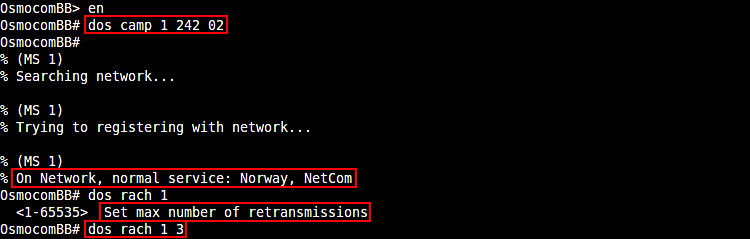
\includegraphics[width=\textwidth]{mobile_dos_rach}
        \caption{Using the \prog{dos rach} command: sending three Channel
        Request messages to \comp{Netcom}}
        \label{fig:mobile_dos_rach}
      \end{figure}

      \begin{figure}[p]
        \centering
        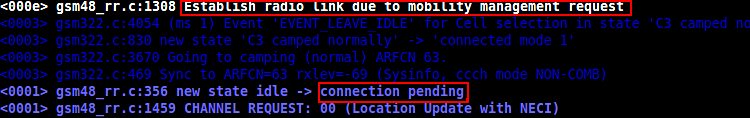
\includegraphics[width=\textwidth]{log_dos_rach}
        \caption{Using the \prog{dos rach} command: the MS tries to
        establish a radio link.}
        \label{fig:log_dos_rach}
      \end{figure}

      \begin{figure}[p]
        \centering
        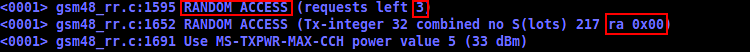
\includegraphics[width=\textwidth]{log_dos_rach2}
        \caption{Using the \prog{dos rach} command: the MS sends 3
          Random Access messages. This one has a RA of \code{0x00}.}
        \label{fig:log_dos_rach2}
      \end{figure}

      \begin{figure}[p]
        \centering
        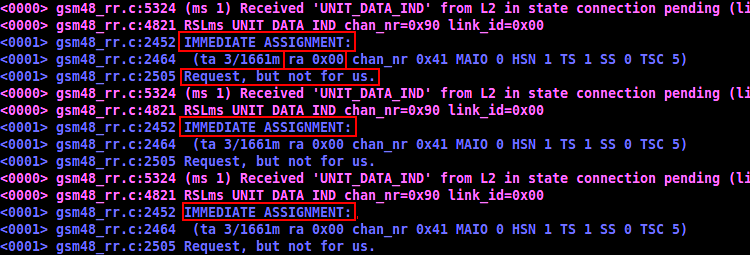
\includegraphics[width=\textwidth]{log_dos_rach3}
        \caption{Using the \prog{dos rach} command: the MS sees
        Immediate Assignment messages with an RA of \code{0x00}, but
      discards them.}
        \label{fig:log_dos_rach3}
      \end{figure}

      \iffalse
      \begin{figure}[p]
        \centering
        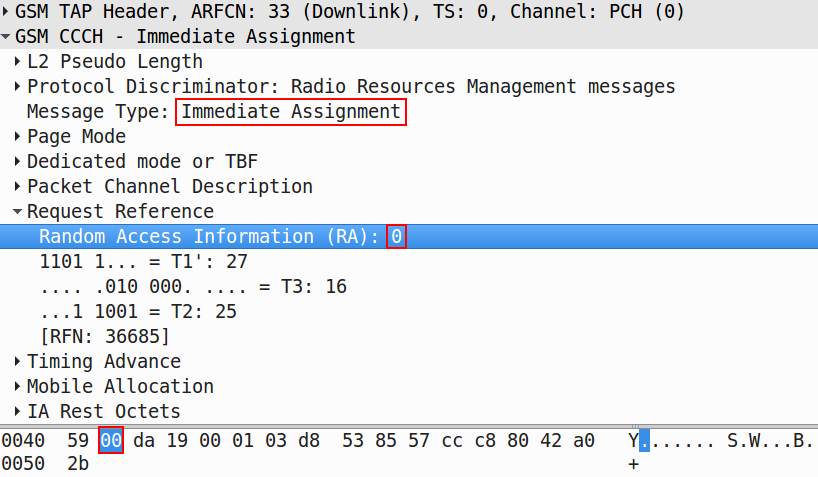
\includegraphics[width=\textwidth]{log_dos_rach4}
        \caption{The MS sees Immediate Assignment messages with an RA
        of \code{0x00}, but discards them. Same in Wireshark.}
        \label{fig:log_dos_rach4}
      \end{figure}
      \fi
   
    \section{IMSI attach flood}

    \iffalse

http://www.etsi.org/deliver/etsi_ts/129000_129099/129002/12.07.00_60/ts_129002v120700p.pdf
look at page 480 for a flow diagram of the whole location update
procedure!!!


    \fi
      \subsection{Theory}

      The \gls{imsi} attach flood attack was introduced at Black Hat
      2010 by \name{the grugq}~\cite{the_grugq_base_2010}. It is almost
      as simple as the previous one, but its impact is much bigger as it
      floods the \gls{vlr} and might flood the \gls{hlr} as well. It
      takes place just after the channel assignment described in the
      previous section. Indeed, when an \gls{ms} wants to attach to a
      network, it requests a channel and starts the \gls{imsi} attach
      procedure, during which the network will require the \gls{ms} to
      identify. The abuse actually happens during the authentication
      procedure, which is not required to succeed.

      The \gls{imsi} attach procedure is described
      in~\Sref{sec:mm_proc_spec} but is summarized here. After
      requesting a channel, the \gls{ms} will send a Location Updating
      Request message to the network. Among other things, it contains
      the identity claimed by the \gls{ms}. Upon reception of the
      message, the network will start the authentication procedure to
      check whether the identity provided by the \gls{ms} can attach to
      the network or not. To do so, the \gls{vlr} will have to look for
      authentication sets related to that identity. If it can not find
      any, it will have to ask the \gls{hlr}. If the identity is not
      found, the network will answer with a Location Updating Reject
      message. If it is found, the network will send an Authentication
      Request message.

      The attack consists of flooding the \gls{vlr} with Location
      Updating Request messages containing random \gls{imsi} values. It
      does not matter if the network sends back Location Updating Reject
      messages, as long as it spends some resources to answer the
      request. If this attack succeeds, it makes the authentication back
      end unavailable. Thus, calls could still be made, but identity
      requests as well as rekeying procedures would fail for the whole
      location area if the \gls{vlr} fails, or for the whole network if
      the \gls{hlr} fails.

      \subsection{Implementation}

      The implementation of the \gls{imsi} attach flood attack created
      for this thesis is based on the \prog{mobile} application of
      \proj{OsmocomBB} again. This application provides a \prog{sim
      testcard} command allowing to create a software \gls{sim} with an
      arbitrary \gls{mcc} and \gls{mnc}. Inserting a new \gls{sim}
      triggers the \gls{imsi} attach procedure to the related network.
      When this happens, a dedicated channel is established, and the
      \gls{ms} sends a Location Updating Request message to the network.
      If the procedure fails, a timer is started with a value of
      \SI{15}{\second}. When the timer elapses, the procedure is started
      again. This is done until the \gls{ms} receives a Location
      Updating Accept or Reject message, or until a given number of
      attempts is reached, three in this case.

      The attack is implemented with three modifications to the
      \prog{mobile} application. The first modification prevents the
      \gls{ms} to act on the reception of Location Updating Reject
      messages. This makes the location updating procedure fail, and
      starts a new procedure when the dedicated timer elapses. The
      second modification significantly decreases the value of that
      timer. The third modification sets a new random \gls{imsi}
      belonging to the targeted network to every new Location Updating
      Request message.

      The result is a continuous flow of Location Updating messages with
      different \glspl{imsi}. This attack is started with the \prog{dos
      attach} command which can be added to the \prog{mobile}
      application with the patch available in \Sref{app:patches} in the
      appendices.

      \subsection{Demonstration}

      The use of the \prog{dos attach} command in the \prog{mobile}
      interface is shown on \fref{fig:mobile_dos_attach}. The arguments
      are the \gls{mcc}, the \gls{mnc}, and the retry delay in seconds.
      This example shows Location Update attempts every \SI{60}{\second}
      on \comp{Netcom}. Again, this does not perform a \gls{dos} attack,
      since the goal is not to damage the network. An usual retry delay
      is much shorter: around \SI{15}{\second}. The \gls{imsi} used during
      the procedure is random, but its \gls{mcc} and \gls{mnc} belong to
      the targeted network. 

      \fref{fig:log_dos_attach2} shows the impact of the command on the
      logs of the \prog{mobile} application. The \gls{ms} establishes a
      dedicated channel, then sends a Location Updating message.
      \fref{fig:log_dos_attach4} shows how the location updating
      procedure fails, and how the timer was changed to
      \SI{60}{\second}.

      \begin{figure}[p]
        \centering
        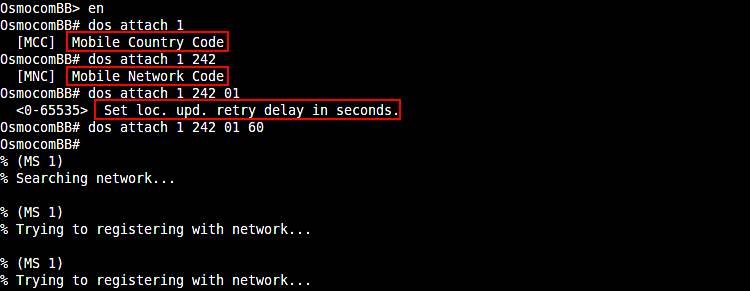
\includegraphics[width=\textwidth]{mobile_dos_attach}
        \caption{Using the \prog{dos attach} command: sending Location
        Updating messages every \SI{60}{\second} on \comp{Netcom}, using
      a random IMSI which could belong to this operator.}
        \label{fig:mobile_dos_attach}
      \end{figure}

      \iffalse
      \begin{figure}[p]
        \centering
        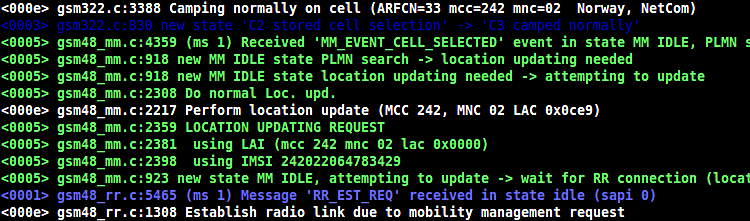
\includegraphics[width=\textwidth]{log_dos_attach}
        \caption{Using the \prog{dos attach} to send a Location Updating
          Request with a random IMSI to \comp{Netcom} using Wireshark.}
        \label{fig:log_dos_attach}
      \end{figure}
      \fi

      \begin{figure}[p]
        \centering
        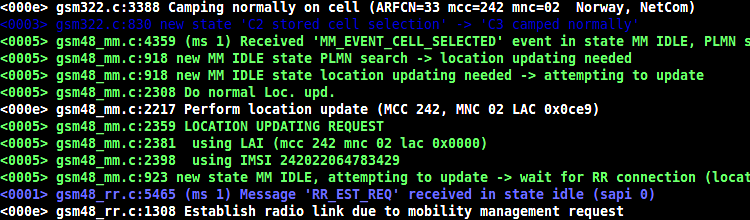
\includegraphics[width=\textwidth]{log_dos_attach2}
        \caption{Using the \prog{dos attach} command: the location
        updating procedure is initiated with a random IMSI on
      \comp{Netcom}.}
        \label{fig:log_dos_attach2}
      \end{figure}

      \iffalse
      \begin{figure}[p]
        \centering
        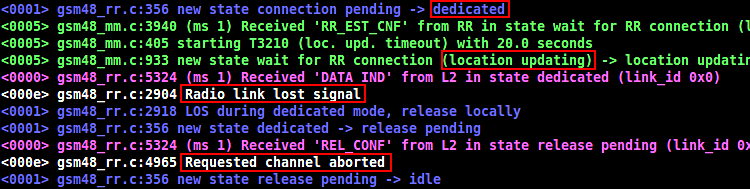
\includegraphics[width=\textwidth]{log_dos_attach3}
        \caption{Using the \prog{dos attach} command: the connection is
          aborted as soon as any message is received.\fxnote{Should wait
            until rejected actually, so that the vlr does some work.}}
        \label{fig:log_dos_attach3}
      \end{figure}
      \fi

      \begin{figure}[p]
        \centering
        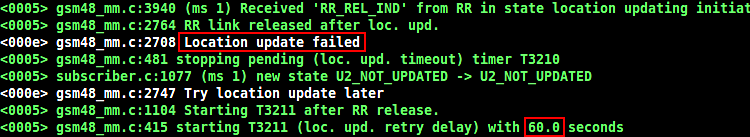
\includegraphics[width=\textwidth]{log_dos_attach4}
        \caption{Using the \prog{dos attach} command: the location updating procedure failed, start again in
        60 seconds.}
        \label{fig:log_dos_attach4}
      \end{figure}


    \section{IMSI detach}

      \subsection{Theory}

      The third attack was first demonstrated by \name{Sylvain Munaut}
      at DeepSec 2010~\cite{munaut_cheap_2010}. It exploits the lack of
      authentication for the \gls{imsi} detach procedure. Again, this
      attack is very simple to implement, since the attacker needs to
      send one single message, but it requires an extra step: an
      \gls{hlr} query. It is more subtle than the previous ones, and can
      target a single \gls{ms}. An analysis of this attack was also
      performed by \name{Elena Recas de
      Buen}~\cite{recas_de_buen_security_2011}.

      The \gls{imsi} detach procedure is used when a subscriber wants to
      detach from the network, for example when the \gls{ms} is shutting
      down. In this case, after opening a channel, the \gls{ms} sends an
      IMSI Detach Indication message containing its identity, \gls{tmsi}
      or \gls{imsi}, to the network. Then, the network will mark this
      identity as detached in the \gls{vlr} without requiring
      authentication or sending any acknowledgement back to the
      \gls{ms}, and terminate any connection with it. More information
      on this procedure is available in~\Sref{sec:mm_proc_com}.

      Of course, this message can be exploited. If the identity of the
      targeted phone on the network is known, for example through an
      \gls{hlr} query, an attacker can disrupt any call and prevent any
      mobile-terminated services by detaching the target from the
      network. The targeted \gls{ms} will receive any \gls{sms} or
      voice mail messages as soon as it registers to the network again.
      Thus, if the targeted phone is actively trying to request a
      service, the attacker has to send an IMSI Detach Indication
      regularly to interrupt the newly established connection. 

      Supporting the IMSI Detach Indication is an optional procedure for
      the operators. Indeed, it might happen that the network does not
      receive a legitimate message without the user knowing it, since
      there is no acknowledgement. In this case, the network only
      notices that the subscriber is not available when the planned
      periodic location update is not executed. So, operators can
      prevent this attack by rejecting any IMSI Detach Indication
      message, and rely on periodic location updates to know when the
      subscriber is not available. Operators can also make it harder for
      attackers by only accepting IMSI Detach Indication containing an
      identity as a \gls{tmsi}. Indeed, a legitimate phone detaching
      from the network would always have a \gls{tmsi}, since it is
      currently attached.

      \subsection{Implementation}

      Again, the implementation of the \gls{imsi} detach attack created
      for this thesis is based on the \prog{mobile} application of
      \proj{OsmocomBB}. Using a simple \gls{imsi} detach procedure
      provided by this application is not practical for two reasons.
      Firstly, it can only be started when the phone is camping on a
      network and able to provide normal service. Secondly, the \gls{ms}
      is turned off at the end of this procedure. To solve the first
      issue, the \prog{dos camp} command introduced
      in~\Sref{sec:rachell_impl} is used. The second issue is solved by
      creating the \prog{dos detach} command which sends an \gls{imsi}
      Detach Indication message without starting the \gls{imsi} detach
      procedure. This is available in the patch provided in
      \Sref{app:patches} in the appendices, and an example is shown on
      \fref{fig:mobile_dos_detach}.

      \subsection{Demonstration}

      An example of the \prog{dos detach} command usage is shown on
      \fref{fig:mobile_dos_detach}. Is shows the only argument: the
      targeted \gls{imsi}. In this case, the \gls{imsi} belongs to
      \comp{Telenor}, but is fake. \fref{fig:mobile_dos_detach} shows
      the message being sent with the specified \gls{imsi}.

      \begin{figure}[h]
        \centering
        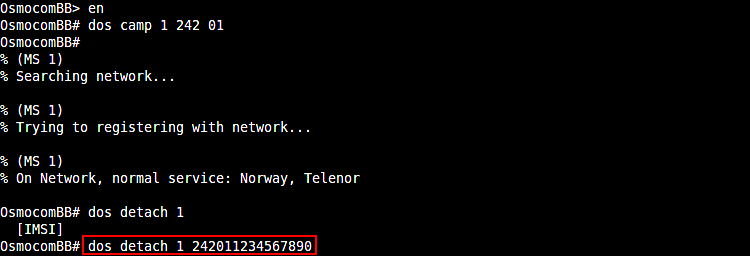
\includegraphics[width=\textwidth]{mobile_dos_detach}
        \caption{Using the \prog{dos detach} command: sending an IMSI
        Detach Indication message with the IMSI 242011234567890 on
      \comp{Telenor}}
        \label{fig:mobile_dos_detach}
      \end{figure}

      \begin{figure}[h]
        \centering
        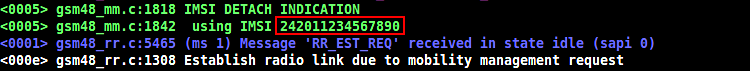
\includegraphics[width=\textwidth]{log_dos_detach}
        \caption{Using the \prog{dos detach} command: an IMSI
          Detach Indication message is sent on \comp{Telenor} with the IMSI 242011234567890}
        \label{fig:mobile_dos_detach}
      \end{figure}

      \iffalse
      \begin{figure}[h]
        \centering
        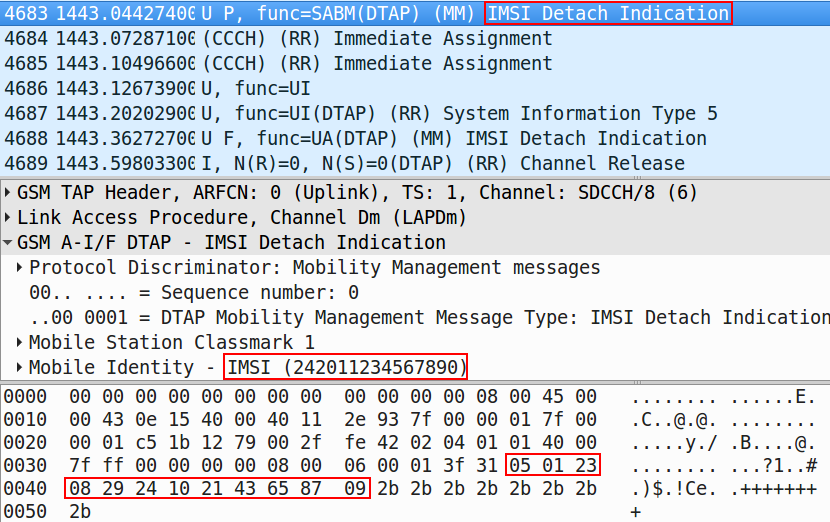
\includegraphics[width=\textwidth]{log_dos_detach1}
        \caption{Using the \prog{dos detach} command: to send an IMSI
        Detach Indication message with the IMSI 242011234567890 on
      \comp{Telenor}. In Wireshark.}
        \label{fig:mobile_dos_detach1}
      \end{figure}

      \begin{figure}[h]
        \centering
        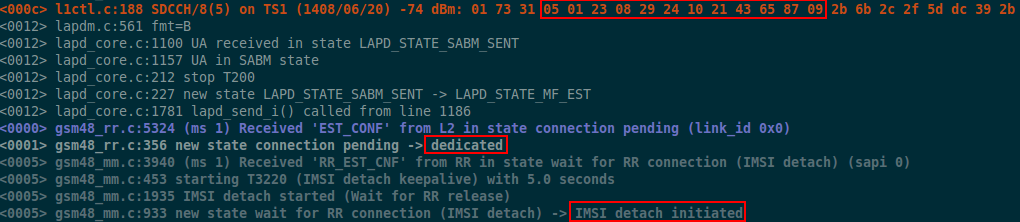
\includegraphics[width=\textwidth]{log_dos_detach2}
        \caption{Can see the message being sent, and the connection being
        established. l1ctl is shown before gsm48 but sent before.}
        \label{fig:mobile_dos_detach2}
      \end{figure}
      \fi


    \section{Paging race condition}

      \subsection{Theory}

      This last attack was demonstrated at the 29C3 by \name{Nico
      Golde}, who worked on that topic with \name{Kevin Redon}, and
      \name{Jean-Pierre Seifert}~\cite{golde_let_2013,golde_let_2012}.
      It exploits the response time of most mobile phones to Paging
      Request messages and is therefore difficult to prevent for the
      operator. It can target from one subscriber to an entire location
      area, is effective on mobile-terminated services only, and
      requires the attacker to be in the same location area as the
      target.

      This attack exploits the paging procedure, which is explained in
      \Sref{sec:rr_proc}. If the attacker answers to Paging Request
      messages faster than the legitimate target, and if it does not
      have access to the legitimate subscriber authentication
      information, the network will release the connection. Therefore,
      the \gls{sms} messages will not be delivered, and the calls will
      be dropped. The difficult part of the attack is to be faster than
      other phones.

      If the goal is to deny service to a specific set of subscribers,
      knowing their \gls{tmsi} is needed. Explanations on how to find it
      are available in \Sref{sec:recovering_tmsi}. Once the set of
      \gls{tmsi} is known, the attacker can answer the related Paging
      Request messages as fast as possible. If the goal is to deny
      service to a whole location area, the attacker can follow as many
      Immediate Assignment messages as possible, using as many modified
      phones as possible, and does not need to know any \gls{tmsi}. It
      is also possible to combine this attack with an IMSI detach attack
      by sending IMSI Detach Indication messages to all the paged
      \gls{tmsi}. It is then important to answer to the Paging Request
      messages first to prevent the targeted phones from attaching to the
      network again.

      Finally, it would also be possible to hijack a mobile-terminated
      service using the same method. If the attacker can win the race
      condition and knows the session key, it is possible to receive a
      service that was intended to the targeted phone, like an \gls{sms}
      message, or a phone call. More information on the ways to find a
      session key are found in \Sref{sec:finding_kc}.

      \subsection{Implementation}

      It would be easy to use the \prog{sim testcard} command of the
      \prog{mobile} application provided with \proj{OsmocomBB} to set a
      fake \gls{mcc}, \gls{mnc}, \gls{lac}, and \gls{tmsi}. This would
      make the phone follow any paging request dedicated to that
      identity. However, the difficulty of this attack is to answer
      faster than the legitimate user, and this can probably not be done
      using the \prog{mobile} application.
      
      A fast implementation of this attack was published by \name{Nico
      Golde} and \name{Kevin Redon} but was not tested in the scope of
      this thesis~\cite{golde_paging_2013, golde_let_2013-1}.  By
      stripping \proj{OsmocomBB} from everything not related to the
      paging procedure, and by running the rest on the baseband
      processor instead of running it on the host computer, it is
      possible to have a very quick answer time. According to the source
      code, it seems to allow a \gls{dos} for a given \gls{tmsi}, for a
      range of \glspl{tmsi}, or for a whole location area. It also
      provides a proof of concept for an \gls{sms} stealing feature.


      \iffalse
      https://www.troopers.de/wp-content/uploads/2012/12/TROOPERS13-Attacking_mobile-terminated_services_in_GSM-Nico_Golde.pdf
      http://users.sec.t-labs.tu-berlin.de/~nico/fun_with_paging_4f0acac4c1fa538082f54cb14bef0841aa9c8abb.diff
      https://tinyurl.com/fun-with-paging

      (Uncleaned) source code available:
      http://tinyurl.com/fun-with-paging
      
      Apply on osmocom changeset 
      4f0acac4c1fa538082f54cb14bef0841aa9c8abb
      \fi
